\Subsection{Augmenting GUI Models with Feature Instantiations}
\label{sec:modelAugmentation}

Given a GUI model $G = \langle V, E, r, A, \mathcal{L} \rangle$ of the target app and a library $\mathcal{F}$ of interaction features, specified as discussed in Section~\ref{sec:featureDefinition}, the next step in our approach is to annotate $G$ with all possible instantiations of each feature in $\mathcal{F}$ to produce an augmented GUI model $G^+ = \langle V, E^+, r, A^+, \mathcal{L}^+ \rangle$. Specifically, this involves adding a set of special labeled edges, called \textit{golden edges}, to $G$. Each golden edge, $e_f(v_1, v_2)$ denotes that feature $f$ when exercised at the state of vertex $v_1$ takes the application to the state of vertex $v_2$. Further, $e_f$ is labeled with $\mathbf{u}_f$, the action sequence of feature $f$. Thus, the augmented model $G^+$ includes the augmented set of edges $E^+ = E \cup E_{golden}$,  augmented action set $A^+ = A \cup \bigcup_{f \in \mathcal{F}} \mathbf{u}_f$, and appropriately modified labeling function $\mathcal{L}^+: A^+ \rightarrow E^+$, where $E_{golden}$ are the golden edges and $\bigcup_{f \in \mathcal{F}} \mathbf{u}_f$ are the actions for features $\mathcal{F}$ labeling the golden edges.

\begin{algorithm}[t]
\begin{footnotesize}
  \DontPrintSemicolon
  \SetAlFnt{\scriptsize\scriptfont}
  \SetKwData{Left}{left}\SetKwData{This}{this}\SetKwData{Up}{up}
  \SetKwFunction{Union}{Union}\SetKwFunction{FindCompress}{FindCompress}
  \SetKwInOut{Input}{Input}\SetKwInOut{Output}{Output}
  \caption{GUI Model Augmentation Algorithm}\label{alg:augmentGUImodel}
  \Input{$G = \langle V, E, r, A, \mathcal{L} \rangle$: Original GUI model of target app \\
  	$\mathcal{F}$: Feature library
  }
  \Output{$G^+ = \langle V, E^+, r, A^+, \mathcal{L}^+ \rangle$: Augmented GUI model}
  \BlankLine
  \Begin{
  		$G^+ \leftarrow G$\;
  		\ForEach{$v \in V$}{
  			\tcp{Iterate over each vertex (state) of $G$}
  			\ForEach{$f \in \mathcal{F}$}{
  				\tcp{Iterate over each feature in $\mathcal{F}$}
  				$dSet = \mathit{destinationSet}(v, G^+, f) $\;
  				\ForEach{$v_1 \in dSet$}{
  					$e \leftarrow \mathit{createEdge}(v, v_1);$\;
  					$\mathit{setEdgeLabel}(e, getAction(f))$\;
  					$\mathit{markGolden}(e)$\;
  					$\mathit{addEdge}(e, G^+)$\;
  				}
  			}
  		}
			\Return{$G^+$}\;
  }
\end{footnotesize}  
\end{algorithm}

Algorithm~\ref{alg:augmentGUImodel} shows the procedure to perform GUI model augmentation. The algorithm iterates over each state $v$ in the GUI model (lines $3-13$) and each feature $f$ in library $\mathcal{F}$, instantiating $f$ at $v$, as per the feature definition. It computes the set of possible destination vertices $dSet$, by evaluating function $D_f$ in the feature definition (function $\mathit{destinationSet()}$ on line $5$). It then iterates over each possible destination vertex $v_1$ (lines $6-11$) creating and adding a golden edge, labeled by the feature's action sequence $\mathbf{u}_f$ (line $8$), to the augmented model $G^+$.
Figure~\ref{fig:dotGraph} shows the GUI model of our simplified version of Kitchen Timer from Section~\ref{example}, augmented with golden edges for the Double Rotation and Back button features.

\begin{figure*}[!t]
\centering
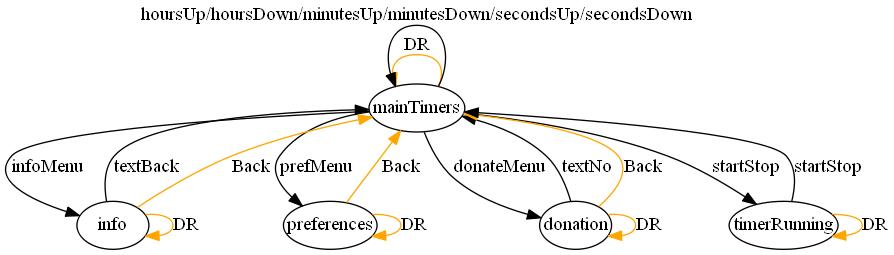
\includegraphics[width=0.65\textwidth]{figures/dotGraph.jpg}
\Caption{Simplified Model of Kitchen Timer.}
\label{fig:dotGraph}
\end{figure*}
